\documentclass[twoside]{book}

% Packages required by doxygen
\usepackage{calc}
\usepackage{doxygen}
\usepackage{graphicx}
\usepackage[utf8]{inputenc}
\usepackage{makeidx}
\usepackage{multicol}
\usepackage{multirow}
\usepackage{textcomp}
\usepackage[table]{xcolor}

% NLS support packages
Portuguese
% Font selection
\usepackage[T1]{fontenc}
\usepackage{mathptmx}
\usepackage[scaled=.90]{helvet}
\usepackage{courier}
\usepackage{amssymb}
\usepackage{sectsty}
\renewcommand{\familydefault}{\sfdefault}
\allsectionsfont{%
  \fontseries{bc}\selectfont%
  \color{darkgray}%
}
\renewcommand{\DoxyLabelFont}{%
  \fontseries{bc}\selectfont%
  \color{darkgray}%
}

% Page & text layout
\usepackage{geometry}
\geometry{%
  a4paper,%
  top=2.5cm,%
  bottom=2.5cm,%
  left=2.5cm,%
  right=2.5cm%
}
\tolerance=750
\hfuzz=15pt
\hbadness=750
\setlength{\emergencystretch}{15pt}
\setlength{\parindent}{0cm}
\setlength{\parskip}{0.2cm}
\makeatletter
\renewcommand{\paragraph}{%
  \@startsection{paragraph}{4}{0ex}{-1.0ex}{1.0ex}{%
    \normalfont\normalsize\bfseries\SS@parafont%
  }%
}
\renewcommand{\subparagraph}{%
  \@startsection{subparagraph}{5}{0ex}{-1.0ex}{1.0ex}{%
    \normalfont\normalsize\bfseries\SS@subparafont%
  }%
}
\makeatother

% Headers & footers
\usepackage{fancyhdr}
\pagestyle{fancyplain}
\fancyhead[LE]{\fancyplain{}{\bfseries\thepage}}
\fancyhead[CE]{\fancyplain{}{}}
\fancyhead[RE]{\fancyplain{}{\bfseries\leftmark}}
\fancyhead[LO]{\fancyplain{}{\bfseries\rightmark}}
\fancyhead[CO]{\fancyplain{}{}}
\fancyhead[RO]{\fancyplain{}{\bfseries\thepage}}
\fancyfoot[LE]{\fancyplain{}{}}
\fancyfoot[CE]{\fancyplain{}{}}
\fancyfoot[RE]{\fancyplain{}{\bfseries\scriptsize Gerado em Quarta, 11 de Setembro de 2013 11\-:12\-:56 para Estrutura de Dados por Doxygen }}
\fancyfoot[LO]{\fancyplain{}{\bfseries\scriptsize Gerado em Quarta, 11 de Setembro de 2013 11\-:12\-:56 para Estrutura de Dados por Doxygen }}
\fancyfoot[CO]{\fancyplain{}{}}
\fancyfoot[RO]{\fancyplain{}{}}
\renewcommand{\footrulewidth}{0.4pt}
\renewcommand{\chaptermark}[1]{%
  \markboth{#1}{}%
}
\renewcommand{\sectionmark}[1]{%
  \markright{\thesection\ #1}%
}

% Indices & bibliography
\usepackage{natbib}
\usepackage[titles]{tocloft}
\setcounter{tocdepth}{3}
\setcounter{secnumdepth}{5}
\makeindex

% Hyperlinks (required, but should be loaded last)
\usepackage{ifpdf}
\ifpdf
  \usepackage[pdftex,pagebackref=true]{hyperref}
\else
  \usepackage[ps2pdf,pagebackref=true]{hyperref}
\fi
\hypersetup{%
  colorlinks=true,%
  linkcolor=blue,%
  citecolor=blue,%
  unicode%
}

% Custom commands
\newcommand{\clearemptydoublepage}{%
  \newpage{\pagestyle{empty}\cleardoublepage}%
}


%===== C O N T E N T S =====

\begin{document}

% Titlepage & ToC
\hypersetup{pageanchor=false}
\pagenumbering{roman}
\begin{titlepage}
\vspace*{7cm}
\begin{center}%
{\Large Estrutura de Dados \\[1ex]\large 1.\-6 }\\
\vspace*{1cm}
{\large Gerado por Doxygen 1.8.5}\\
\vspace*{0.5cm}
{\small Quarta, 11 de Setembro de 2013 11:12:56}\\
\end{center}
\end{titlepage}
\clearemptydoublepage
\tableofcontents
\clearemptydoublepage
\pagenumbering{arabic}
\hypersetup{pageanchor=true}

%--- Begin generated contents ---
\chapter{Página principal}
\label{index}\hypertarget{index}{}Trabalho desenvolvido para aprendizado do conteúdo da disciplina Estrutura de Dados. 
\chapter{Índice da hierarquia}
\section{Hierarquia de classes}
Esta lista de heranças está organizada, dentro do possível, por ordem alfabética\-:\begin{DoxyCompactList}
\item \contentsline{section}{Estrutura\-De\-Dados$<$ Tipo $>$}{\pageref{classEstruturaDeDados}}{}
\begin{DoxyCompactList}
\item \contentsline{section}{E\-D\-Linear$<$ Tipo $>$}{\pageref{classEDLinear}}{}
\begin{DoxyCompactList}
\item \contentsline{section}{Fila$<$ Tipo $>$}{\pageref{classFila}}{}
\item \contentsline{section}{Lista$<$ Tipo $>$}{\pageref{classLista}}{}
\item \contentsline{section}{Pilha$<$ Tipo $>$}{\pageref{classPilha}}{}
\end{DoxyCompactList}
\end{DoxyCompactList}
\item \contentsline{section}{Estrutura\-De\-Dados$<$ char $\ast$ $>$}{\pageref{classEstruturaDeDados}}{}
\begin{DoxyCompactList}
\item \contentsline{section}{E\-D\-Linear$<$ char $\ast$ $>$}{\pageref{classEDLinear}}{}
\begin{DoxyCompactList}
\item \contentsline{section}{Lista$<$ char $\ast$ $>$}{\pageref{classLista}}{}
\begin{DoxyCompactList}
\item \contentsline{section}{Lista\-Char}{\pageref{classListaChar}}{}
\end{DoxyCompactList}
\end{DoxyCompactList}
\end{DoxyCompactList}
\item \contentsline{section}{Estrutura\-De\-Dados$<$ Lancamento $>$}{\pageref{classEstruturaDeDados}}{}
\begin{DoxyCompactList}
\item \contentsline{section}{E\-D\-Linear$<$ Lancamento $>$}{\pageref{classEDLinear}}{}
\begin{DoxyCompactList}
\item \contentsline{section}{Lista$<$ Lancamento $>$}{\pageref{classLista}}{}
\begin{DoxyCompactList}
\item \contentsline{section}{Lista\-Contabil}{\pageref{classListaContabil}}{}
\end{DoxyCompactList}
\end{DoxyCompactList}
\end{DoxyCompactList}
\item \contentsline{section}{Fachada\-Pilha}{\pageref{classFachadaPilha}}{}
\item \contentsline{section}{Informa\-Dados}{\pageref{classInformaDados}}{}
\item \contentsline{section}{Lancamento}{\pageref{classLancamento}}{}
\item \contentsline{section}{Produto}{\pageref{classProduto}}{}
\item \contentsline{section}{Recebe\-Dados}{\pageref{classRecebeDados}}{}
\end{DoxyCompactList}

\chapter{Índice dos componentes}
\section{Lista de componentes}
Lista de classes, estruturas, uniões e interfaces com uma breve descrição\-:\begin{DoxyCompactList}
\item\contentsline{section}{\hyperlink{classEDLinear}{E\-D\-Linear$<$ Tipo $>$} }{\pageref{classEDLinear}}{}
\item\contentsline{section}{\hyperlink{classEstruturaDeDados}{Estrutura\-De\-Dados$<$ Tipo $>$} }{\pageref{classEstruturaDeDados}}{}
\item\contentsline{section}{\hyperlink{classFachadaPilha}{Fachada\-Pilha} }{\pageref{classFachadaPilha}}{}
\item\contentsline{section}{\hyperlink{classFila}{Fila$<$ Tipo $>$} }{\pageref{classFila}}{}
\item\contentsline{section}{\hyperlink{classInformaDados}{Informa\-Dados} }{\pageref{classInformaDados}}{}
\item\contentsline{section}{\hyperlink{classLista}{Lista$<$ Tipo $>$} }{\pageref{classLista}}{}
\item\contentsline{section}{\hyperlink{classPilha}{Pilha$<$ Tipo $>$} }{\pageref{classPilha}}{}
\item\contentsline{section}{\hyperlink{classRecebeDados}{Recebe\-Dados} }{\pageref{classRecebeDados}}{}
\end{DoxyCompactList}

\chapter{Documentação da classe}
\hypertarget{classEDLinear}{\section{Referência à classe Template E\-D\-Linear$<$ Tipo $>$}
\label{classEDLinear}\index{E\-D\-Linear$<$ Tipo $>$@{E\-D\-Linear$<$ Tipo $>$}}
}
Diagrama de heranças da classe E\-D\-Linear$<$ Tipo $>$\begin{figure}[H]
\begin{center}
\leavevmode
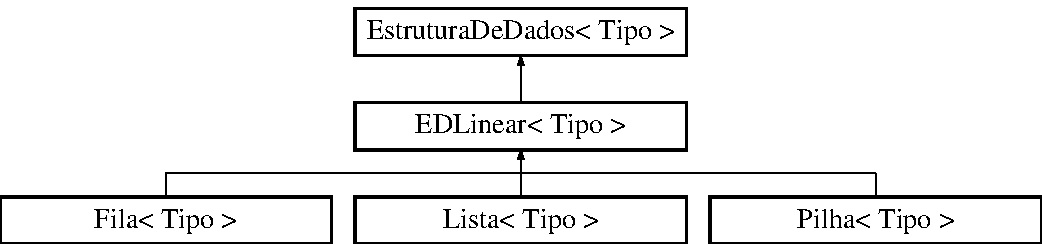
\includegraphics[height=3.000000cm]{classEDLinear}
\end{center}
\end{figure}
\subsection*{Membros públicos}
\begin{DoxyCompactItemize}
\item 
void \hyperlink{classEDLinear_af867a99c232007c2c11fd84cdbe603d3}{adicionar} (Tipo t)
\begin{DoxyCompactList}\small\item\em Adiciona elemento na estrutura de dados. \end{DoxyCompactList}\item 
int \hyperlink{classEDLinear_a5f36413e1900ef421dfbed681f303675}{tamanho} ()
\begin{DoxyCompactList}\small\item\em Informa tamanho da lista. \end{DoxyCompactList}\item 
bool \hyperlink{classEDLinear_a29e7eaef660cda7d95897917b1b1973f}{vazia} ()
\begin{DoxyCompactList}\small\item\em Informa se lista está vazia. \end{DoxyCompactList}\item 
bool \hyperlink{classEDLinear_a8187f3ef636dc2d82e84fa10dc27456d}{cheia} ()
\begin{DoxyCompactList}\small\item\em Informa se lista está cheia. \end{DoxyCompactList}\item 
\hypertarget{classEDLinear_ae57113a1f9b4b63f73aeea99deda939d}{void {\bfseries limpar} ()}\label{classEDLinear_ae57113a1f9b4b63f73aeea99deda939d}

\end{DoxyCompactItemize}
\subsection*{Atributos Protegidos}
\begin{DoxyCompactItemize}
\item 
\hypertarget{classEDLinear_aa8d44a073aaccf250998e7f938aed24f}{Tipo {\bfseries arr} \mbox{[}M\-A\-X\mbox{]}}\label{classEDLinear_aa8d44a073aaccf250998e7f938aed24f}

\item 
\hypertarget{classEDLinear_a1b1bb258f72504bfb71a326fead1ce14}{int {\bfseries topo}}\label{classEDLinear_a1b1bb258f72504bfb71a326fead1ce14}

\end{DoxyCompactItemize}


\subsection{Descrição detalhada}
\subsubsection*{template$<$typename Tipo$>$class E\-D\-Linear$<$ Tipo $>$}



Definido na linha 6 do ficheiro E\-D\-Linear.\-h.



\subsection{Documentação dos métodos}
\hypertarget{classEDLinear_af867a99c232007c2c11fd84cdbe603d3}{\index{E\-D\-Linear@{E\-D\-Linear}!adicionar@{adicionar}}
\index{adicionar@{adicionar}!EDLinear@{E\-D\-Linear}}
\subsubsection[{adicionar}]{\setlength{\rightskip}{0pt plus 5cm}template$<$typename Tipo $>$ void {\bf E\-D\-Linear}$<$ Tipo $>$\-::adicionar (
\begin{DoxyParamCaption}
\item[{Tipo}]{t}
\end{DoxyParamCaption}
)\hspace{0.3cm}{\ttfamily [inline]}, {\ttfamily [virtual]}}}\label{classEDLinear_af867a99c232007c2c11fd84cdbe603d3}


Adiciona elemento na estrutura de dados. 


\begin{DoxyParams}{Parâmetros}
{\em t} & é o elemento que será adicionado à estrutura\\
\hline
\end{DoxyParams}
\begin{DoxyReturn}{Retorna}
void
\end{DoxyReturn}
\begin{DoxyRemark}{Observações}
Essa função não pode ser chamada com a estrutura cheia 
\end{DoxyRemark}


Implementa \hyperlink{classEstruturaDeDados_a66bd359407b52b76b5be611ef25cf847}{Estrutura\-De\-Dados$<$ Tipo $>$}.



Definido na linha 18 do ficheiro E\-D\-Linear.\-h.

\hypertarget{classEDLinear_a8187f3ef636dc2d82e84fa10dc27456d}{\index{E\-D\-Linear@{E\-D\-Linear}!cheia@{cheia}}
\index{cheia@{cheia}!EDLinear@{E\-D\-Linear}}
\subsubsection[{cheia}]{\setlength{\rightskip}{0pt plus 5cm}template$<$typename Tipo $>$ bool {\bf E\-D\-Linear}$<$ Tipo $>$\-::cheia (
\begin{DoxyParamCaption}
{}
\end{DoxyParamCaption}
)\hspace{0.3cm}{\ttfamily [inline]}, {\ttfamily [virtual]}}}\label{classEDLinear_a8187f3ef636dc2d82e84fa10dc27456d}


Informa se lista está cheia. 

\begin{DoxyReturn}{Retorna}
true se lista estiver cheia 
\end{DoxyReturn}


Implementa \hyperlink{classEstruturaDeDados_a5d7866e13c2e6129e42979093569348c}{Estrutura\-De\-Dados$<$ Tipo $>$}.



Definido na linha 33 do ficheiro E\-D\-Linear.\-h.

\hypertarget{classEDLinear_a5f36413e1900ef421dfbed681f303675}{\index{E\-D\-Linear@{E\-D\-Linear}!tamanho@{tamanho}}
\index{tamanho@{tamanho}!EDLinear@{E\-D\-Linear}}
\subsubsection[{tamanho}]{\setlength{\rightskip}{0pt plus 5cm}template$<$typename Tipo $>$ int {\bf E\-D\-Linear}$<$ Tipo $>$\-::tamanho (
\begin{DoxyParamCaption}
{}
\end{DoxyParamCaption}
)\hspace{0.3cm}{\ttfamily [inline]}, {\ttfamily [virtual]}}}\label{classEDLinear_a5f36413e1900ef421dfbed681f303675}


Informa tamanho da lista. 

\begin{DoxyReturn}{Retorna}
Inteiro representando o tamanho da lista 
\end{DoxyReturn}


Implementa \hyperlink{classEstruturaDeDados_aedcdd78aed7517cfad5ddbe374d7ce88}{Estrutura\-De\-Dados$<$ Tipo $>$}.



Definido na linha 25 do ficheiro E\-D\-Linear.\-h.

\hypertarget{classEDLinear_a29e7eaef660cda7d95897917b1b1973f}{\index{E\-D\-Linear@{E\-D\-Linear}!vazia@{vazia}}
\index{vazia@{vazia}!EDLinear@{E\-D\-Linear}}
\subsubsection[{vazia}]{\setlength{\rightskip}{0pt plus 5cm}template$<$typename Tipo $>$ bool {\bf E\-D\-Linear}$<$ Tipo $>$\-::vazia (
\begin{DoxyParamCaption}
{}
\end{DoxyParamCaption}
)\hspace{0.3cm}{\ttfamily [inline]}, {\ttfamily [virtual]}}}\label{classEDLinear_a29e7eaef660cda7d95897917b1b1973f}


Informa se lista está vazia. 

\begin{DoxyReturn}{Retorna}
true se lista estiver vazia 
\end{DoxyReturn}


Implementa \hyperlink{classEstruturaDeDados_aa45fc3c6284cba7c27b9cd128e71a079}{Estrutura\-De\-Dados$<$ Tipo $>$}.



Definido na linha 29 do ficheiro E\-D\-Linear.\-h.



A documentação para esta classe foi gerada a partir do seguinte ficheiro\-:\begin{DoxyCompactItemize}
\item 
Trabalho\-E\-D/src/include/E\-D\-Linear.\-h\end{DoxyCompactItemize}

\hypertarget{classEstruturaDeDados}{\section{Referência à classe Template Estrutura\-De\-Dados$<$ Tipo $>$}
\label{classEstruturaDeDados}\index{Estrutura\-De\-Dados$<$ Tipo $>$@{Estrutura\-De\-Dados$<$ Tipo $>$}}
}
Diagrama de heranças da classe Estrutura\-De\-Dados$<$ Tipo $>$\begin{figure}[H]
\begin{center}
\leavevmode
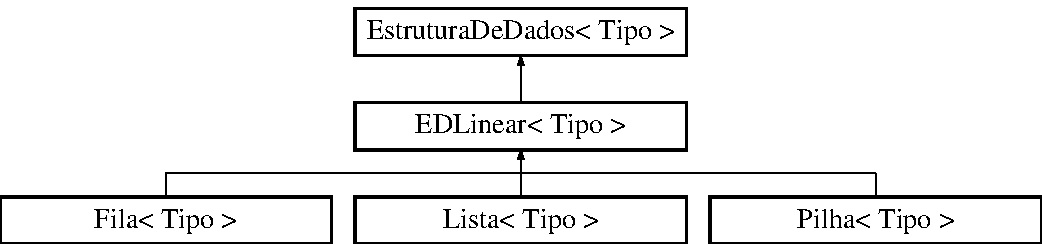
\includegraphics[height=3.000000cm]{classEstruturaDeDados}
\end{center}
\end{figure}
\subsection*{Membros públicos}
\begin{DoxyCompactItemize}
\item 
virtual void \hyperlink{classEstruturaDeDados_a66bd359407b52b76b5be611ef25cf847}{adicionar} (Tipo t)=0
\begin{DoxyCompactList}\small\item\em Adiciona elemento na estrutura de dados. \end{DoxyCompactList}\item 
virtual Tipo \hyperlink{classEstruturaDeDados_a01ddc5aec2e4a425e4021055c15e7f02}{remover} ()=0
\begin{DoxyCompactList}\small\item\em Remove elemento da estrutura de dados. \end{DoxyCompactList}\item 
virtual int \hyperlink{classEstruturaDeDados_aedcdd78aed7517cfad5ddbe374d7ce88}{tamanho} ()=0
\begin{DoxyCompactList}\small\item\em Informa tamanho da lista. \end{DoxyCompactList}\item 
virtual bool \hyperlink{classEstruturaDeDados_a5d7866e13c2e6129e42979093569348c}{cheia} ()=0
\begin{DoxyCompactList}\small\item\em Informa se lista está cheia. \end{DoxyCompactList}\item 
virtual bool \hyperlink{classEstruturaDeDados_aa45fc3c6284cba7c27b9cd128e71a079}{vazia} ()=0
\begin{DoxyCompactList}\small\item\em Informa se lista está vazia. \end{DoxyCompactList}\end{DoxyCompactItemize}


\subsection{Descrição detalhada}
\subsubsection*{template$<$typename Tipo$>$class Estrutura\-De\-Dados$<$ Tipo $>$}



Definido na linha 2 do ficheiro Estrutura\-De\-Dados.\-h.



\subsection{Documentação dos métodos}
\hypertarget{classEstruturaDeDados_a66bd359407b52b76b5be611ef25cf847}{\index{Estrutura\-De\-Dados@{Estrutura\-De\-Dados}!adicionar@{adicionar}}
\index{adicionar@{adicionar}!EstruturaDeDados@{Estrutura\-De\-Dados}}
\subsubsection[{adicionar}]{\setlength{\rightskip}{0pt plus 5cm}template$<$typename Tipo $>$ virtual void {\bf Estrutura\-De\-Dados}$<$ Tipo $>$\-::adicionar (
\begin{DoxyParamCaption}
\item[{Tipo}]{t}
\end{DoxyParamCaption}
)\hspace{0.3cm}{\ttfamily [pure virtual]}}}\label{classEstruturaDeDados_a66bd359407b52b76b5be611ef25cf847}


Adiciona elemento na estrutura de dados. 


\begin{DoxyParams}{Parâmetros}
{\em t} & é o elemento que será adicionado à estrutura\\
\hline
\end{DoxyParams}
\begin{DoxyReturn}{Retorna}
void
\end{DoxyReturn}
\begin{DoxyRemark}{Observações}
Essa função não pode ser chamada com a estrutura cheia 
\end{DoxyRemark}


Implementado em \hyperlink{classEDLinear_af867a99c232007c2c11fd84cdbe603d3}{E\-D\-Linear$<$ Tipo $>$}.

\hypertarget{classEstruturaDeDados_a5d7866e13c2e6129e42979093569348c}{\index{Estrutura\-De\-Dados@{Estrutura\-De\-Dados}!cheia@{cheia}}
\index{cheia@{cheia}!EstruturaDeDados@{Estrutura\-De\-Dados}}
\subsubsection[{cheia}]{\setlength{\rightskip}{0pt plus 5cm}template$<$typename Tipo $>$ virtual bool {\bf Estrutura\-De\-Dados}$<$ Tipo $>$\-::cheia (
\begin{DoxyParamCaption}
{}
\end{DoxyParamCaption}
)\hspace{0.3cm}{\ttfamily [pure virtual]}}}\label{classEstruturaDeDados_a5d7866e13c2e6129e42979093569348c}


Informa se lista está cheia. 

\begin{DoxyReturn}{Retorna}
true se lista estiver cheia 
\end{DoxyReturn}


Implementado em \hyperlink{classEDLinear_a8187f3ef636dc2d82e84fa10dc27456d}{E\-D\-Linear$<$ Tipo $>$}.

\hypertarget{classEstruturaDeDados_a01ddc5aec2e4a425e4021055c15e7f02}{\index{Estrutura\-De\-Dados@{Estrutura\-De\-Dados}!remover@{remover}}
\index{remover@{remover}!EstruturaDeDados@{Estrutura\-De\-Dados}}
\subsubsection[{remover}]{\setlength{\rightskip}{0pt plus 5cm}template$<$typename Tipo $>$ virtual Tipo {\bf Estrutura\-De\-Dados}$<$ Tipo $>$\-::remover (
\begin{DoxyParamCaption}
{}
\end{DoxyParamCaption}
)\hspace{0.3cm}{\ttfamily [pure virtual]}}}\label{classEstruturaDeDados_a01ddc5aec2e4a425e4021055c15e7f02}


Remove elemento da estrutura de dados. 

\begin{DoxyReturn}{Retorna}
Elemento retirado da estrutura
\end{DoxyReturn}
\begin{DoxyRemark}{Observações}
Essa função não pode ser chamada com a estrutura vazia 
\end{DoxyRemark}


Implementado em \hyperlink{classLista_a58768c31b7137a2303212b63e9804dc6}{Lista$<$ Tipo $>$}, \hyperlink{classPilha_a57d9edb93b911f91b4527f7ab365ef8c}{Pilha$<$ Tipo $>$} e \hyperlink{classFila_a687d9d8738e4aabeed0d7025e26d36d5}{Fila$<$ Tipo $>$}.

\hypertarget{classEstruturaDeDados_aedcdd78aed7517cfad5ddbe374d7ce88}{\index{Estrutura\-De\-Dados@{Estrutura\-De\-Dados}!tamanho@{tamanho}}
\index{tamanho@{tamanho}!EstruturaDeDados@{Estrutura\-De\-Dados}}
\subsubsection[{tamanho}]{\setlength{\rightskip}{0pt plus 5cm}template$<$typename Tipo $>$ virtual int {\bf Estrutura\-De\-Dados}$<$ Tipo $>$\-::tamanho (
\begin{DoxyParamCaption}
{}
\end{DoxyParamCaption}
)\hspace{0.3cm}{\ttfamily [pure virtual]}}}\label{classEstruturaDeDados_aedcdd78aed7517cfad5ddbe374d7ce88}


Informa tamanho da lista. 

\begin{DoxyReturn}{Retorna}
Inteiro representando o tamanho da lista 
\end{DoxyReturn}


Implementado em \hyperlink{classEDLinear_a5f36413e1900ef421dfbed681f303675}{E\-D\-Linear$<$ Tipo $>$}.

\hypertarget{classEstruturaDeDados_aa45fc3c6284cba7c27b9cd128e71a079}{\index{Estrutura\-De\-Dados@{Estrutura\-De\-Dados}!vazia@{vazia}}
\index{vazia@{vazia}!EstruturaDeDados@{Estrutura\-De\-Dados}}
\subsubsection[{vazia}]{\setlength{\rightskip}{0pt plus 5cm}template$<$typename Tipo $>$ virtual bool {\bf Estrutura\-De\-Dados}$<$ Tipo $>$\-::vazia (
\begin{DoxyParamCaption}
{}
\end{DoxyParamCaption}
)\hspace{0.3cm}{\ttfamily [pure virtual]}}}\label{classEstruturaDeDados_aa45fc3c6284cba7c27b9cd128e71a079}


Informa se lista está vazia. 

\begin{DoxyReturn}{Retorna}
true se lista estiver vazia 
\end{DoxyReturn}


Implementado em \hyperlink{classEDLinear_a29e7eaef660cda7d95897917b1b1973f}{E\-D\-Linear$<$ Tipo $>$}.



A documentação para esta classe foi gerada a partir do seguinte ficheiro\-:\begin{DoxyCompactItemize}
\item 
Trabalho\-E\-D/src/include/Estrutura\-De\-Dados.\-h\end{DoxyCompactItemize}

\hypertarget{classFachadaPilha}{\section{Referência à classe Fachada\-Pilha}
\label{classFachadaPilha}\index{Fachada\-Pilha@{Fachada\-Pilha}}
}
\subsection*{Membros públicos}
\begin{DoxyCompactItemize}
\item 
void \hyperlink{classFachadaPilha_a82efe2889afb6eb2345a651eaa7206b5}{chama\-Pilha} ()
\begin{DoxyCompactList}\small\item\em Serve de intermédio entre o modelo lógico da pilha e a entrada de dados. \end{DoxyCompactList}\end{DoxyCompactItemize}


\subsection{Descrição detalhada}


Definido na linha 1 do ficheiro Fachada\-Pilha.\-h.



\subsection{Documentação dos métodos}
\hypertarget{classFachadaPilha_a82efe2889afb6eb2345a651eaa7206b5}{\index{Fachada\-Pilha@{Fachada\-Pilha}!chama\-Pilha@{chama\-Pilha}}
\index{chama\-Pilha@{chama\-Pilha}!FachadaPilha@{Fachada\-Pilha}}
\subsubsection[{chama\-Pilha}]{\setlength{\rightskip}{0pt plus 5cm}void Fachada\-Pilha\-::chama\-Pilha (
\begin{DoxyParamCaption}
{}
\end{DoxyParamCaption}
)}}\label{classFachadaPilha_a82efe2889afb6eb2345a651eaa7206b5}


Serve de intermédio entre o modelo lógico da pilha e a entrada de dados. 

\begin{DoxyReturn}{Retorna}
void 
\end{DoxyReturn}


Definido na linha 10 do ficheiro Fachada\-Pilha.\-cpp.



A documentação para esta classe foi gerada a partir dos seguintes ficheiros\-:\begin{DoxyCompactItemize}
\item 
Trabalho\-E\-D/src/include/Fachada\-Pilha.\-h\item 
Trabalho\-E\-D/src/Fachada\-Pilha.\-cpp\end{DoxyCompactItemize}

\hypertarget{classFila}{\section{Referência à classe Template Fila$<$ Tipo $>$}
\label{classFila}\index{Fila$<$ Tipo $>$@{Fila$<$ Tipo $>$}}
}
Diagrama de heranças da classe Fila$<$ Tipo $>$\begin{figure}[H]
\begin{center}
\leavevmode
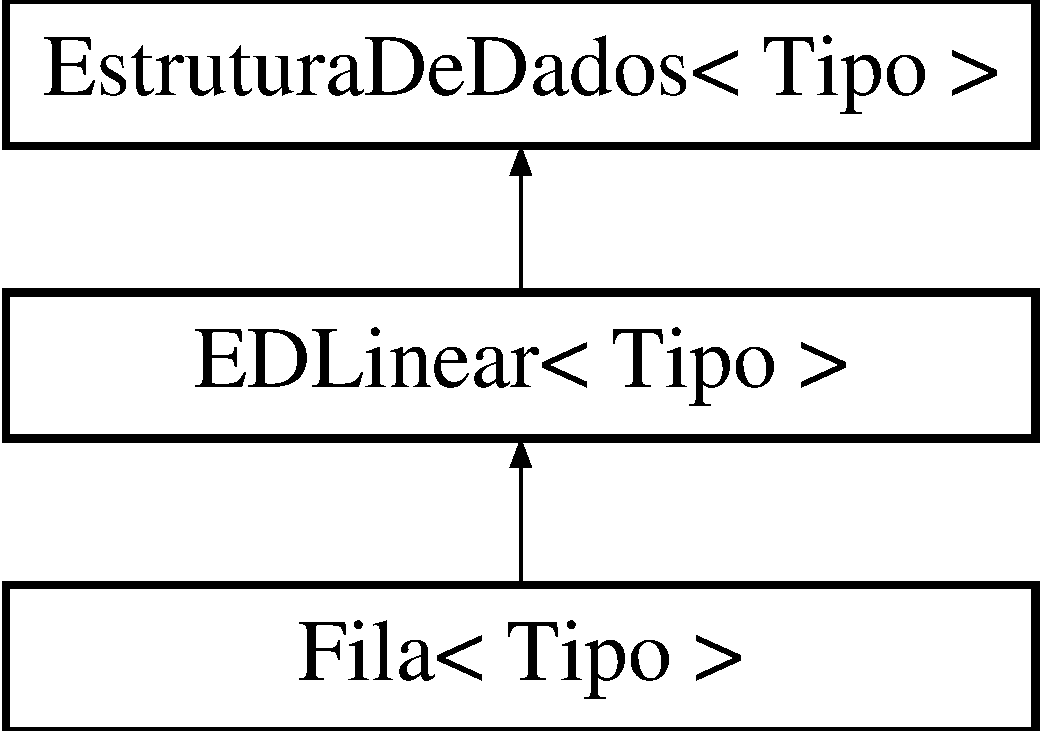
\includegraphics[height=3.000000cm]{classFila}
\end{center}
\end{figure}
\subsection*{Membros públicos}
\begin{DoxyCompactItemize}
\item 
Tipo \hyperlink{classFila_a687d9d8738e4aabeed0d7025e26d36d5}{remover} ()
\begin{DoxyCompactList}\small\item\em Remove elemento da estrutura de dados. \end{DoxyCompactList}\end{DoxyCompactItemize}
\subsection*{Additional Inherited Members}


\subsection{Descrição detalhada}
\subsubsection*{template$<$typename Tipo$>$class Fila$<$ Tipo $>$}



Definido na linha 7 do ficheiro Fila.\-h.



\subsection{Documentação dos métodos}
\hypertarget{classFila_a687d9d8738e4aabeed0d7025e26d36d5}{\index{Fila@{Fila}!remover@{remover}}
\index{remover@{remover}!Fila@{Fila}}
\subsubsection[{remover}]{\setlength{\rightskip}{0pt plus 5cm}template$<$typename Tipo $>$ Tipo {\bf Fila}$<$ Tipo $>$\-::remover (
\begin{DoxyParamCaption}
{}
\end{DoxyParamCaption}
)\hspace{0.3cm}{\ttfamily [inline]}, {\ttfamily [virtual]}}}\label{classFila_a687d9d8738e4aabeed0d7025e26d36d5}


Remove elemento da estrutura de dados. 

\begin{DoxyReturn}{Retorna}
Elemento retirado da estrutura
\end{DoxyReturn}
\begin{DoxyRemark}{Observações}
Essa função não pode ser chamada com a estrutura vazia 
\end{DoxyRemark}


Implementa \hyperlink{classEstruturaDeDados_a01ddc5aec2e4a425e4021055c15e7f02}{Estrutura\-De\-Dados$<$ Tipo $>$}.



Definido na linha 14 do ficheiro Fila.\-h.



A documentação para esta classe foi gerada a partir do seguinte ficheiro\-:\begin{DoxyCompactItemize}
\item 
repositorio/\-Trabalho\-E\-D/src/include/Fila.\-h\end{DoxyCompactItemize}

\hypertarget{classInformaDados}{\section{Referência à classe Informa\-Dados}
\label{classInformaDados}\index{Informa\-Dados@{Informa\-Dados}}
}
\subsection*{Membros públicos}
\begin{DoxyCompactItemize}
\item 
\hypertarget{classInformaDados_aadd413615e51e0bf6d5b9b644b625b46}{void {\bfseries exibe\-String} (string s)}\label{classInformaDados_aadd413615e51e0bf6d5b9b644b625b46}

\item 
\hypertarget{classInformaDados_a906587453c1b5c5ac6105d74ae1c23ef}{void {\bfseries exibe\-Inteiro} (int $\ast$i)}\label{classInformaDados_a906587453c1b5c5ac6105d74ae1c23ef}

\end{DoxyCompactItemize}


\subsection{Descrição detalhada}


Definido na linha 5 do ficheiro Informa\-Dados.\-h.



A documentação para esta classe foi gerada a partir dos seguintes ficheiros\-:\begin{DoxyCompactItemize}
\item 
Trabalho\-E\-D/src/include/Informa\-Dados.\-h\item 
Trabalho\-E\-D/src/Informa\-Dados.\-cpp\end{DoxyCompactItemize}

\hypertarget{classLancamento}{\section{Referência à classe Lancamento}
\label{classLancamento}\index{Lancamento@{Lancamento}}
}
\subsection*{Membros públicos}
\begin{DoxyCompactItemize}
\item 
\hypertarget{classLancamento_abbab3e9ae6b8ee0090c2e905df8ce444}{{\bfseries Lancamento} (char $\ast$n, double p)}\label{classLancamento_abbab3e9ae6b8ee0090c2e905df8ce444}

\item 
double \hyperlink{classLancamento_ac2015e1a0e422b7e6df888f0875bf1ae}{get\-Valor} ()
\begin{DoxyCompactList}\small\item\em Retorna valor do lançamento. \end{DoxyCompactList}\item 
char $\ast$ \hyperlink{classLancamento_a20fc96ffe2c8e4169427b52ece18286d}{get\-Nome} ()
\begin{DoxyCompactList}\small\item\em Retorna ponteiro para primeira posição do nome do lançamento. \end{DoxyCompactList}\item 
\hyperlink{classLancamento_add3c84ee103af2d2f01e658a7ff36d3f}{Lancamento} (const \hyperlink{classLancamento}{Lancamento} \&outro)
\begin{DoxyCompactList}\small\item\em Construtor de cópia do lançamento. \end{DoxyCompactList}\end{DoxyCompactItemize}


\subsection{Descrição detalhada}


Definido na linha 1 do ficheiro Lancamento.\-h.



\subsection{Documentação dos Construtores \& Destrutor}
\hypertarget{classLancamento_add3c84ee103af2d2f01e658a7ff36d3f}{\index{Lancamento@{Lancamento}!Lancamento@{Lancamento}}
\index{Lancamento@{Lancamento}!Lancamento@{Lancamento}}
\subsubsection[{Lancamento}]{\setlength{\rightskip}{0pt plus 5cm}Lancamento\-::\-Lancamento (
\begin{DoxyParamCaption}
\item[{const {\bf Lancamento} \&}]{outro}
\end{DoxyParamCaption}
)}}\label{classLancamento_add3c84ee103af2d2f01e658a7ff36d3f}


Construtor de cópia do lançamento. 


\begin{DoxyParams}{Parâmetros}
{\em outro} & é o objeto \hyperlink{classLancamento}{Lancamento} a ser copiado \\
\hline
\end{DoxyParams}


Definido na linha 25 do ficheiro Lancamento.\-cpp.



\subsection{Documentação dos métodos}
\hypertarget{classLancamento_a20fc96ffe2c8e4169427b52ece18286d}{\index{Lancamento@{Lancamento}!get\-Nome@{get\-Nome}}
\index{get\-Nome@{get\-Nome}!Lancamento@{Lancamento}}
\subsubsection[{get\-Nome}]{\setlength{\rightskip}{0pt plus 5cm}char $\ast$ Lancamento\-::get\-Nome (
\begin{DoxyParamCaption}
{}
\end{DoxyParamCaption}
)}}\label{classLancamento_a20fc96ffe2c8e4169427b52ece18286d}


Retorna ponteiro para primeira posição do nome do lançamento. 

\begin{DoxyReturn}{Retorna}
$\ast$char 
\end{DoxyReturn}


Definido na linha 21 do ficheiro Lancamento.\-cpp.

\hypertarget{classLancamento_ac2015e1a0e422b7e6df888f0875bf1ae}{\index{Lancamento@{Lancamento}!get\-Valor@{get\-Valor}}
\index{get\-Valor@{get\-Valor}!Lancamento@{Lancamento}}
\subsubsection[{get\-Valor}]{\setlength{\rightskip}{0pt plus 5cm}double Lancamento\-::get\-Valor (
\begin{DoxyParamCaption}
{}
\end{DoxyParamCaption}
)}}\label{classLancamento_ac2015e1a0e422b7e6df888f0875bf1ae}


Retorna valor do lançamento. 

\begin{DoxyReturn}{Retorna}
double 
\end{DoxyReturn}


Definido na linha 17 do ficheiro Lancamento.\-cpp.



A documentação para esta classe foi gerada a partir dos seguintes ficheiros\-:\begin{DoxyCompactItemize}
\item 
repositorio/\-Trabalho\-E\-D/src/include/Lancamento.\-h\item 
repositorio/\-Trabalho\-E\-D/src/Lancamento.\-cpp\end{DoxyCompactItemize}

\hypertarget{classLista}{\section{Referência à classe Template Lista$<$ Tipo $>$}
\label{classLista}\index{Lista$<$ Tipo $>$@{Lista$<$ Tipo $>$}}
}
Diagrama de heranças da classe Lista$<$ Tipo $>$\begin{figure}[H]
\begin{center}
\leavevmode
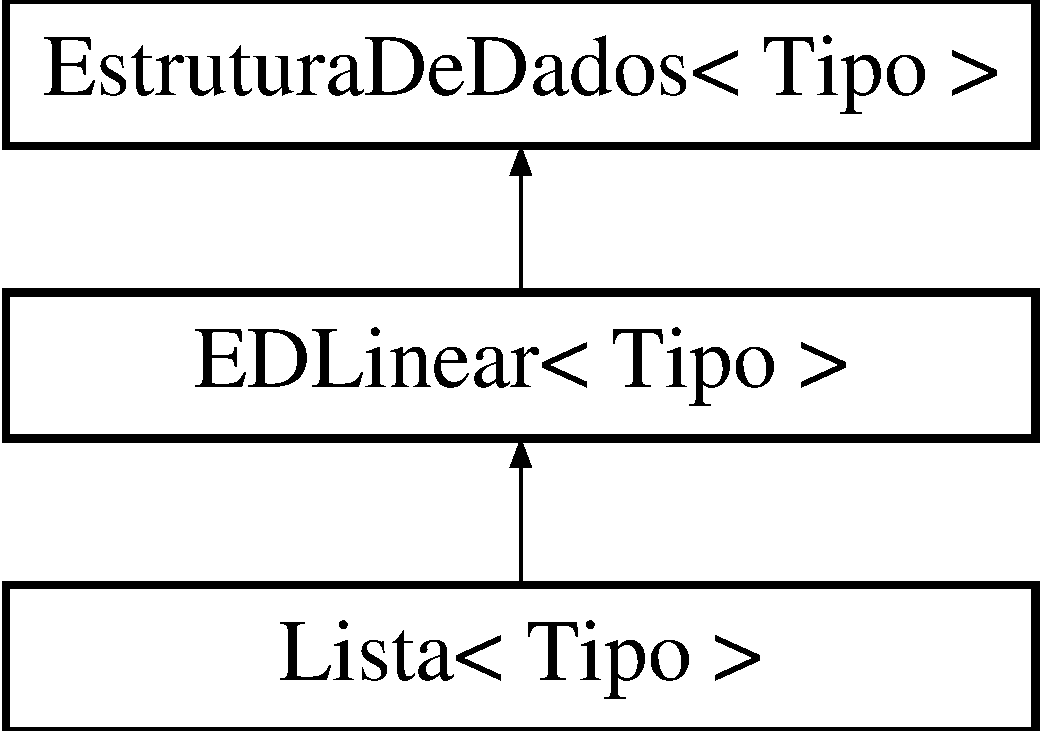
\includegraphics[height=3.000000cm]{classLista}
\end{center}
\end{figure}
\subsection*{Membros públicos}
\begin{DoxyCompactItemize}
\item 
\hypertarget{classLista_a21853f382bab3540ab6dfeece9fe3ba1}{void {\bfseries adiciona\-Na\-Posicao} (Tipo t, int posicao)}\label{classLista_a21853f382bab3540ab6dfeece9fe3ba1}

\item 
\hypertarget{classLista_a9c9a9ac8cbf7e849b2e470c3be5926a2}{void {\bfseries adiciona\-Em\-Ordem} (Tipo t)}\label{classLista_a9c9a9ac8cbf7e849b2e470c3be5926a2}

\item 
Tipo \hyperlink{classLista_a58768c31b7137a2303212b63e9804dc6}{remover} ()
\begin{DoxyCompactList}\small\item\em Remove elemento da estrutura de dados. \end{DoxyCompactList}\item 
\hypertarget{classLista_a554cfbab02c678a9186ffb3d80079e97}{Tipo {\bfseries retira\-Da\-Posicao} (int posicao)}\label{classLista_a554cfbab02c678a9186ffb3d80079e97}

\item 
\hypertarget{classLista_a29b4ed24294d84af7e6287374338f868}{void {\bfseries retira\-Especifico} (Tipo t)}\label{classLista_a29b4ed24294d84af7e6287374338f868}

\item 
\hypertarget{classLista_ad374d77a408c513004c79cd33ddc76a3}{int {\bfseries posicao} (Tipo t)}\label{classLista_ad374d77a408c513004c79cd33ddc76a3}

\item 
\hypertarget{classLista_a3dcad88a266c9d487e149c366f7e8d05}{bool {\bfseries contem} (Tipo t)}\label{classLista_a3dcad88a266c9d487e149c366f7e8d05}

\item 
\hypertarget{classLista_a2ffbcb916698dba55a97290ff91be666}{bool {\bfseries igual} (Tipo t1, Tipo t2)}\label{classLista_a2ffbcb916698dba55a97290ff91be666}

\item 
\hypertarget{classLista_a9b265cf31415874bd52170d3ae4abe29}{bool {\bfseries maior} (Tipo t1, Tipo t2)}\label{classLista_a9b265cf31415874bd52170d3ae4abe29}

\item 
\hypertarget{classLista_a4b879b1914f3bf9bc76570a50749aafc}{bool {\bfseries menor} (Tipo t1, Tipo t2)}\label{classLista_a4b879b1914f3bf9bc76570a50749aafc}

\end{DoxyCompactItemize}
\subsection*{Additional Inherited Members}


\subsection{Descrição detalhada}
\subsubsection*{template$<$typename Tipo$>$class Lista$<$ Tipo $>$}



Definido na linha 5 do ficheiro Lista.\-h.



\subsection{Documentação dos métodos}
\hypertarget{classLista_a58768c31b7137a2303212b63e9804dc6}{\index{Lista@{Lista}!remover@{remover}}
\index{remover@{remover}!Lista@{Lista}}
\subsubsection[{remover}]{\setlength{\rightskip}{0pt plus 5cm}template$<$typename Tipo $>$ Tipo {\bf Lista}$<$ Tipo $>$\-::remover (
\begin{DoxyParamCaption}
{}
\end{DoxyParamCaption}
)\hspace{0.3cm}{\ttfamily [inline]}, {\ttfamily [virtual]}}}\label{classLista_a58768c31b7137a2303212b63e9804dc6}


Remove elemento da estrutura de dados. 

\begin{DoxyReturn}{Retorna}
Elemento retirado da estrutura
\end{DoxyReturn}
\begin{DoxyRemark}{Observações}
Essa função não pode ser chamada com a estrutura vazia 
\end{DoxyRemark}


Implementa \hyperlink{classEstruturaDeDados_a01ddc5aec2e4a425e4021055c15e7f02}{Estrutura\-De\-Dados$<$ Tipo $>$}.



Definido na linha 32 do ficheiro Lista.\-h.



A documentação para esta classe foi gerada a partir do seguinte ficheiro\-:\begin{DoxyCompactItemize}
\item 
Trabalho\-E\-D/src/include/Lista.\-h\end{DoxyCompactItemize}

\hypertarget{classListaChar}{\section{Referência à classe Lista\-Char}
\label{classListaChar}\index{Lista\-Char@{Lista\-Char}}
}
Diagrama de heranças da classe Lista\-Char\begin{figure}[H]
\begin{center}
\leavevmode
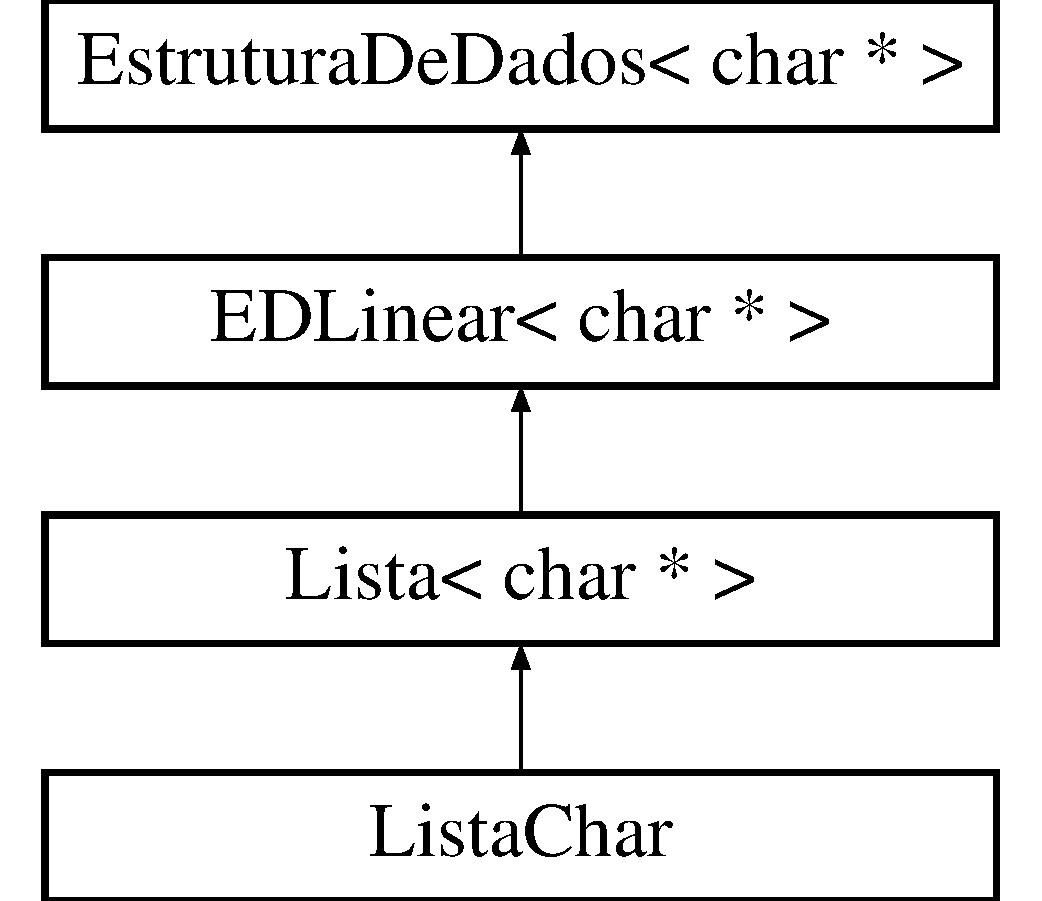
\includegraphics[height=4.000000cm]{classListaChar}
\end{center}
\end{figure}
\subsection*{Additional Inherited Members}


\subsection{Descrição detalhada}


Definido na linha 4 do ficheiro Lista\-Char.\-h.



A documentação para esta classe foi gerada a partir dos seguintes ficheiros\-:\begin{DoxyCompactItemize}
\item 
repositorio/\-Trabalho\-E\-D/src/include/Lista\-Char.\-h\item 
repositorio/\-Trabalho\-E\-D/src/Lista\-Char.\-cpp\end{DoxyCompactItemize}

\hypertarget{classListaContabil}{\section{Referência à classe Lista\-Contabil}
\label{classListaContabil}\index{Lista\-Contabil@{Lista\-Contabil}}
}
Diagrama de heranças da classe Lista\-Contabil\begin{figure}[H]
\begin{center}
\leavevmode
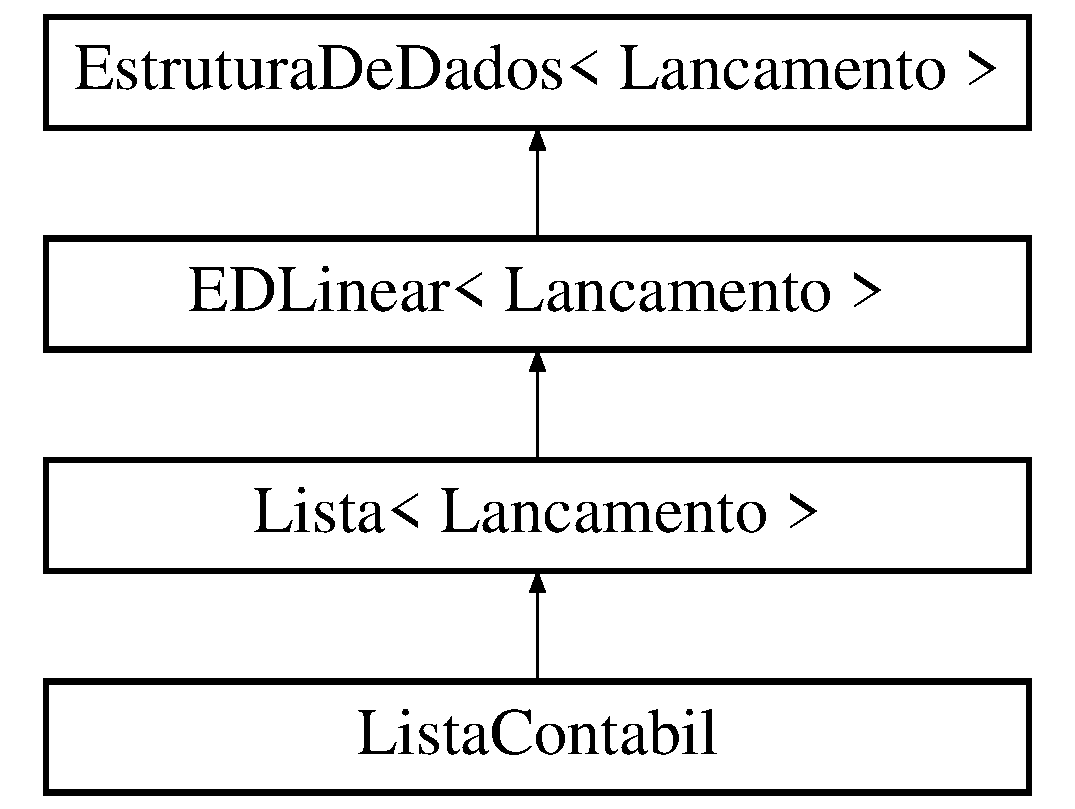
\includegraphics[height=4.000000cm]{classListaContabil}
\end{center}
\end{figure}
\subsection*{Membros públicos}
\begin{DoxyCompactItemize}
\item 
\hyperlink{classLancamento}{Lancamento} \hyperlink{classListaContabil_a8bec61d3afe662507c6ca6ea6db6f973}{mostrar} (int i)
\begin{DoxyCompactList}\small\item\em Retorna objeto lançamento de índice i. \end{DoxyCompactList}\end{DoxyCompactItemize}
\subsection*{Additional Inherited Members}


\subsection{Descrição detalhada}


Definido na linha 4 do ficheiro Lista\-Contabil.\-h.



\subsection{Documentação dos métodos}
\hypertarget{classListaContabil_a8bec61d3afe662507c6ca6ea6db6f973}{\index{Lista\-Contabil@{Lista\-Contabil}!mostrar@{mostrar}}
\index{mostrar@{mostrar}!ListaContabil@{Lista\-Contabil}}
\subsubsection[{mostrar}]{\setlength{\rightskip}{0pt plus 5cm}{\bf Lancamento} Lista\-Contabil\-::mostrar (
\begin{DoxyParamCaption}
\item[{int}]{i}
\end{DoxyParamCaption}
)}}\label{classListaContabil_a8bec61d3afe662507c6ca6ea6db6f973}


Retorna objeto lançamento de índice i. 


\begin{DoxyParams}{Parâmetros}
{\em i} & é o índice\\
\hline
\end{DoxyParams}
\begin{DoxyReturn}{Retorna}
\hyperlink{classLancamento}{Lancamento}
\end{DoxyReturn}
\begin{DoxyRemark}{Observações}
Essa função não pode ser chamada com a estrutura cheia 
\end{DoxyRemark}


Definido na linha 9 do ficheiro Lista\-Contabil.\-cpp.



A documentação para esta classe foi gerada a partir dos seguintes ficheiros\-:\begin{DoxyCompactItemize}
\item 
repositorio/\-Trabalho\-E\-D/src/include/Lista\-Contabil.\-h\item 
repositorio/\-Trabalho\-E\-D/src/Lista\-Contabil.\-cpp\end{DoxyCompactItemize}

\hypertarget{classPilha}{\section{Referência à classe Template Pilha$<$ Tipo $>$}
\label{classPilha}\index{Pilha$<$ Tipo $>$@{Pilha$<$ Tipo $>$}}
}
Diagrama de heranças da classe Pilha$<$ Tipo $>$\begin{figure}[H]
\begin{center}
\leavevmode
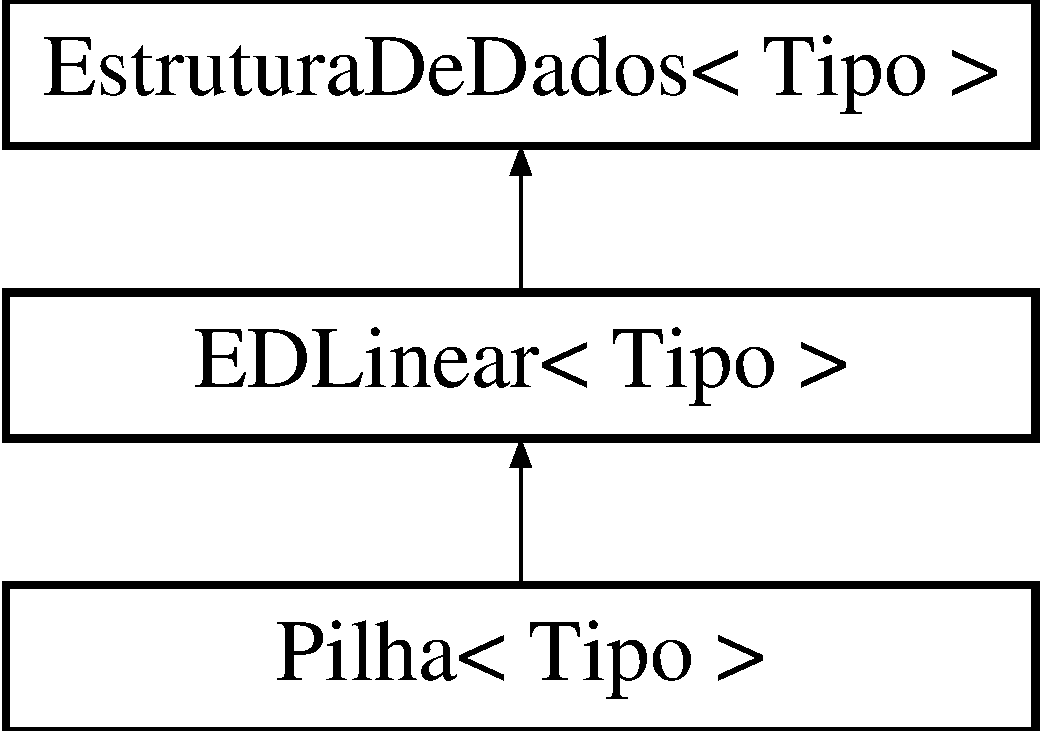
\includegraphics[height=3.000000cm]{classPilha}
\end{center}
\end{figure}
\subsection*{Membros públicos}
\begin{DoxyCompactItemize}
\item 
Tipo \hyperlink{classPilha_a57d9edb93b911f91b4527f7ab365ef8c}{remover} ()
\begin{DoxyCompactList}\small\item\em Remove elemento da estrutura de dados. \end{DoxyCompactList}\end{DoxyCompactItemize}
\subsection*{Additional Inherited Members}


\subsection{Descrição detalhada}
\subsubsection*{template$<$typename Tipo$>$class Pilha$<$ Tipo $>$}



Definido na linha 5 do ficheiro Pilha.\-h.



\subsection{Documentação dos métodos}
\hypertarget{classPilha_a57d9edb93b911f91b4527f7ab365ef8c}{\index{Pilha@{Pilha}!remover@{remover}}
\index{remover@{remover}!Pilha@{Pilha}}
\subsubsection[{remover}]{\setlength{\rightskip}{0pt plus 5cm}template$<$typename Tipo$>$ Tipo {\bf Pilha}$<$ Tipo $>$\-::remover (
\begin{DoxyParamCaption}
{}
\end{DoxyParamCaption}
)\hspace{0.3cm}{\ttfamily [inline]}, {\ttfamily [virtual]}}}\label{classPilha_a57d9edb93b911f91b4527f7ab365ef8c}


Remove elemento da estrutura de dados. 

\begin{DoxyReturn}{Retorna}
Tipo
\end{DoxyReturn}
\begin{DoxyRemark}{Observações}
Essa função lança uma exceção de chamada com a pilha vazia 
\end{DoxyRemark}


Implementa \hyperlink{classEstruturaDeDados_a01ddc5aec2e4a425e4021055c15e7f02}{Estrutura\-De\-Dados$<$ Tipo $>$}.



Definido na linha 20 do ficheiro Pilha.\-h.



A documentação para esta classe foi gerada a partir do seguinte ficheiro\-:\begin{DoxyCompactItemize}
\item 
Trabalho\-E\-D/src/include/Pilha.\-h\end{DoxyCompactItemize}

\hypertarget{classProduto}{\section{Referência à classe Produto}
\label{classProduto}\index{Produto@{Produto}}
}
\subsection*{Membros públicos}
\begin{DoxyCompactItemize}
\item 
\hypertarget{classProduto_af8a28945544529a5bb1b6f5da2e89625}{{\bfseries Produto} (string n, int p)}\label{classProduto_af8a28945544529a5bb1b6f5da2e89625}

\item 
string \hyperlink{classProduto_ab85f6765ddb66a6100c7aa7d7ba379e6}{get\-Nome} ()
\begin{DoxyCompactList}\small\item\em Retorna nome do produto. \end{DoxyCompactList}\item 
int \hyperlink{classProduto_ad646a0dfabe3761ce7f9140db045404c}{get\-Preco} ()
\begin{DoxyCompactList}\small\item\em Retorna preço do produto. \end{DoxyCompactList}\item 
bool \hyperlink{classProduto_ad0983b854c092a1032931693cfa4a915}{operator$<$} (\hyperlink{classProduto}{Produto} \&o)
\begin{DoxyCompactList}\small\item\em Usa preço como critério de comparação. \end{DoxyCompactList}\item 
bool \hyperlink{classProduto_ad39e0021d4c0cd8bf63b669c8000345e}{operator$>$} (\hyperlink{classProduto}{Produto} \&o)
\begin{DoxyCompactList}\small\item\em Usa preço como critério de comparação. \end{DoxyCompactList}\item 
bool \hyperlink{classProduto_a2796bcb084171159ddc67a551c2f1c1e}{operator==} (\hyperlink{classProduto}{Produto} \&o)
\begin{DoxyCompactList}\small\item\em Usa preço como critério de comparação. \end{DoxyCompactList}\end{DoxyCompactItemize}


\subsection{Descrição detalhada}


Definido na linha 5 do ficheiro Produto.\-h.



\subsection{Documentação dos métodos}
\hypertarget{classProduto_ab85f6765ddb66a6100c7aa7d7ba379e6}{\index{Produto@{Produto}!get\-Nome@{get\-Nome}}
\index{get\-Nome@{get\-Nome}!Produto@{Produto}}
\subsubsection[{get\-Nome}]{\setlength{\rightskip}{0pt plus 5cm}string Produto\-::get\-Nome (
\begin{DoxyParamCaption}
{}
\end{DoxyParamCaption}
)}}\label{classProduto_ab85f6765ddb66a6100c7aa7d7ba379e6}


Retorna nome do produto. 

\begin{DoxyReturn}{Retorna}
string 
\end{DoxyReturn}


Definido na linha 16 do ficheiro Produto.\-cpp.

\hypertarget{classProduto_ad646a0dfabe3761ce7f9140db045404c}{\index{Produto@{Produto}!get\-Preco@{get\-Preco}}
\index{get\-Preco@{get\-Preco}!Produto@{Produto}}
\subsubsection[{get\-Preco}]{\setlength{\rightskip}{0pt plus 5cm}int Produto\-::get\-Preco (
\begin{DoxyParamCaption}
{}
\end{DoxyParamCaption}
)}}\label{classProduto_ad646a0dfabe3761ce7f9140db045404c}


Retorna preço do produto. 

\begin{DoxyReturn}{Retorna}
int 
\end{DoxyReturn}


Definido na linha 20 do ficheiro Produto.\-cpp.

\hypertarget{classProduto_ad0983b854c092a1032931693cfa4a915}{\index{Produto@{Produto}!operator$<$@{operator$<$}}
\index{operator$<$@{operator$<$}!Produto@{Produto}}
\subsubsection[{operator$<$}]{\setlength{\rightskip}{0pt plus 5cm}bool Produto\-::operator$<$ (
\begin{DoxyParamCaption}
\item[{{\bf Produto} \&}]{o}
\end{DoxyParamCaption}
)}}\label{classProduto_ad0983b854c092a1032931693cfa4a915}


Usa preço como critério de comparação. 



Definido na linha 24 do ficheiro Produto.\-cpp.

\hypertarget{classProduto_a2796bcb084171159ddc67a551c2f1c1e}{\index{Produto@{Produto}!operator==@{operator==}}
\index{operator==@{operator==}!Produto@{Produto}}
\subsubsection[{operator==}]{\setlength{\rightskip}{0pt plus 5cm}bool Produto\-::operator== (
\begin{DoxyParamCaption}
\item[{{\bf Produto} \&}]{o}
\end{DoxyParamCaption}
)}}\label{classProduto_a2796bcb084171159ddc67a551c2f1c1e}


Usa preço como critério de comparação. 



Definido na linha 32 do ficheiro Produto.\-cpp.

\hypertarget{classProduto_ad39e0021d4c0cd8bf63b669c8000345e}{\index{Produto@{Produto}!operator$>$@{operator$>$}}
\index{operator$>$@{operator$>$}!Produto@{Produto}}
\subsubsection[{operator$>$}]{\setlength{\rightskip}{0pt plus 5cm}bool Produto\-::operator$>$ (
\begin{DoxyParamCaption}
\item[{{\bf Produto} \&}]{o}
\end{DoxyParamCaption}
)}}\label{classProduto_ad39e0021d4c0cd8bf63b669c8000345e}


Usa preço como critério de comparação. 



Definido na linha 28 do ficheiro Produto.\-cpp.



A documentação para esta classe foi gerada a partir dos seguintes ficheiros\-:\begin{DoxyCompactItemize}
\item 
repositorio/\-Trabalho\-E\-D/src/include/Produto.\-h\item 
repositorio/\-Trabalho\-E\-D/src/Produto.\-cpp\end{DoxyCompactItemize}

\hypertarget{classRecebeDados}{\section{Referência à classe Recebe\-Dados}
\label{classRecebeDados}\index{Recebe\-Dados@{Recebe\-Dados}}
}
\subsection*{Membros públicos}
\begin{DoxyCompactItemize}
\item 
int \hyperlink{classRecebeDados_a682a075582832ea6799bf8418459ff64}{pega\-Int} ()
\begin{DoxyCompactList}\small\item\em Recebe um inteiro a partir de entrada de teclado. \end{DoxyCompactList}\item 
std\-::string \hyperlink{classRecebeDados_a8b48e116480d8fbf67ccf813cad17fca}{pega\-String} ()
\begin{DoxyCompactList}\small\item\em Recebe um string a partir de entrada de teclado. \end{DoxyCompactList}\end{DoxyCompactItemize}


\subsection{Descrição detalhada}


Definido na linha 3 do ficheiro Recebe\-Dados.\-h.



\subsection{Documentação dos métodos}
\hypertarget{classRecebeDados_a682a075582832ea6799bf8418459ff64}{\index{Recebe\-Dados@{Recebe\-Dados}!pega\-Int@{pega\-Int}}
\index{pega\-Int@{pega\-Int}!RecebeDados@{Recebe\-Dados}}
\subsubsection[{pega\-Int}]{\setlength{\rightskip}{0pt plus 5cm}int Recebe\-Dados\-::pega\-Int (
\begin{DoxyParamCaption}
{}
\end{DoxyParamCaption}
)}}\label{classRecebeDados_a682a075582832ea6799bf8418459ff64}


Recebe um inteiro a partir de entrada de teclado. 

\begin{DoxyReturn}{Retorna}
int 
\end{DoxyReturn}


Definido na linha 6 do ficheiro Recebe\-Dados.\-cpp.

\hypertarget{classRecebeDados_a8b48e116480d8fbf67ccf813cad17fca}{\index{Recebe\-Dados@{Recebe\-Dados}!pega\-String@{pega\-String}}
\index{pega\-String@{pega\-String}!RecebeDados@{Recebe\-Dados}}
\subsubsection[{pega\-String}]{\setlength{\rightskip}{0pt plus 5cm}string Recebe\-Dados\-::pega\-String (
\begin{DoxyParamCaption}
{}
\end{DoxyParamCaption}
)}}\label{classRecebeDados_a8b48e116480d8fbf67ccf813cad17fca}


Recebe um string a partir de entrada de teclado. 

\begin{DoxyReturn}{Retorna}
string 
\end{DoxyReturn}


Definido na linha 12 do ficheiro Recebe\-Dados.\-cpp.



A documentação para esta classe foi gerada a partir dos seguintes ficheiros\-:\begin{DoxyCompactItemize}
\item 
repositorio/\-Trabalho\-E\-D/src/include/Recebe\-Dados.\-h\item 
repositorio/\-Trabalho\-E\-D/src/Recebe\-Dados.\-cpp\end{DoxyCompactItemize}

%--- End generated contents ---

% Index
\newpage
\phantomsection
\addcontentsline{toc}{part}{Índice}
\printindex

\end{document}
